\documentclass[a4paper,11pt]{report}

\usepackage[T1]{fontenc}
\usepackage[english]{babel}
\usepackage{etoolbox}
\usepackage{sourcecodepro}
\usepackage{amsmath}
\usepackage{amsthm}
\usepackage{fullpage}
\usepackage{bussproofs}
\usepackage{mathpartir}
\usepackage[tableaux]{prooftrees}
\usepackage{algorithmicx}
\usepackage{algpseudocode}
\usepackage{tikz}
\usepackage{array}

\title{Resume : Mathematical Methods for Computer Science}
\author{Sylvain Julmy}

\setlength{\parindent}{0cm}

% For definition, theorem, ...
\newtheorem*{mydef}{Definition}
\newtheorem{theorem}{Theorem}
\newtheorem{corollary}{Corollary}
\newtheorem{lemma}{Lemma}

% Inference rules
\newenvironment{bprooftree}
{\leavevmode\hbox\bgroup}
{\DisplayProof\egroup}

% tikz library
\usetikzlibrary{graphs,graphs.standard}

\begin{document}

\maketitle

\chapter{Combinatorics}
We are counting elements of set :
\begin{gather}
  A \cap B \neq \emptyset \to |A \cup B| = |A| + |B| \\
  |A \times B| = |A| * |B|
\end{gather}

Making two choices independently out of $m$ and $n$ possibilites leads to $m *
n$ different possibilities. For example, throwing a dice twice leads to $6*6=36$
possibilities consecutevely or not.

\begin{gather}
  \underbrace{|A_1 \times \dots \times A_n|}_{|\{(a_1,\dots,a_n), a_i \in A_i\}|} = |A_1| * \dots * |A_n|
\end{gather}

\paragraph{Example : } Throwing $n$ coins leads to $2^n$ possibilities.

Choosing $2$ out of $n$ people is $n(n-1)$.

\begin{gather}
  B \subset A \to |A \setminus B| = |A| - |B|
\end{gather}

\paragraph{Example : } Getting at least one $6$ from two dice : $\frac{6 * 2 - 1}{6*6} \frac{11}{36}$

\section{Quotient rate}

The number of sheep in a herd is equals to the number of legs divided by $4$.

Given a set $A$ with equivalence relation $\sim$ such that every equivalence
class contains $n$ element, we have
\begin{gather}
  |\frac{A}{\sim}| = \frac{|A|}{\sim}
\end{gather}

Have a map $f : x \mapsto y$ such that for every elements of $y$ there are $n$
corresponding elements of $x$, then
\begin{gather}
  |y| = \frac{|x|}{\sim}
\end{gather}

\section{Permutation}

A permutation of a set $A$ is a bijective map $f: A \mapsto A$, where usually $A
= \{1,2,\dots,n\}$.

There are three ways to represent a permutation :

\begin{enumerate}
\item Using a graph-like draw
  \usetikzlibrary{graphs,graphs.standard}
  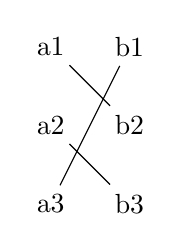
\begin{tikzpicture}[every node/.style={}]
    \graph [simple] {
      a1 -!- b1;
      a2 -!- b2;
      a3 -!- b3;	
      a1 -- b2;
      a2 -- b3;
      a3 -- b1;
    }; 
  \end{tikzpicture}
\item
  \[
    \begin{pmatrix}
      1 & 2 & 3 \\
      f(1) & f(2) & f(3)
    \end{pmatrix}
    =
    \begin{pmatrix}
      1 & 2 & 3 \\
      2 & 3 & 1
    \end{pmatrix}
  \]
\item
  \[
    \begin{pmatrix}
      f(1) & f(2) & f(3)
    \end{pmatrix}
    =
    \begin{pmatrix}
      2 & 3 & 1
    \end{pmatrix}
  \]
\end{enumerate}

There are $n!$ different permutation of the set $\{1,2,\dots,n\}$.

\section{Ordered choice}

Take $k$ out of $n$ element and remember the order, there are
\begin{gather}
  n * (n-1) * \dots * (n - k + 1) = \frac{n!}{(n-k)!}
\end{gather}

number of $k$-permutation in a set of $n$ elements.

\section{Unordered choice}

The number of ways to pick $k$ out of $n$ elements without order is
\[
  \begin{pmatrix} n \\ k\end{pmatrix} = \frac{n!}{(n-k)! \cdot k!}
\]

\begin{theorem}
  \[
    \begin{pmatrix} n \\ k\end{pmatrix} = \begin{pmatrix} n \\ n-k\end{pmatrix}
  \]
\end{theorem}

\begin{proof}
  \begin{align*}
    \begin{pmatrix} n \\ k\end{pmatrix}   &= \frac{n!}{(n-k)! \cdot k!} \\
    \begin{pmatrix} n \\ n-k\end{pmatrix} &= \frac{n!}{(n-(n-k))! \cdot (n-k)!} \\
                                          &= \frac{n!}{k! \cdot (n-k)!}
  \end{align*}
\end{proof}

Number of subset of a set of $n$ element is $ 2^n $. Either we pick an element
or not, so its a sequence of $1$ and $0$ where $1$ means that we pick the
element and $0$ not. Example with $n=5$ : $10010$.

\section{Unordered choices of subsets}

$\begin{pmatrix} n \\ k\end{pmatrix}$ is the number of $k$-elements subsets of
$\{1,2,\dots,n\}$.

\begin{theorem}
  $\begin{pmatrix} n \\ k\end{pmatrix}$ is the number of binary words of length
  $n$ with $k$ digits ``1''.
\end{theorem}

\begin{proof}
  Encode a subset $A \subset \{1,2,\dots,n\}$ by a binary word : $i$th digit is
  ``1'' if $i\in A$ and ``0'' if $i \not \in A$. So binary words with $A$-digit
  ``1'' $\leftrightarrow$ $k$-elements subsets.
\end{proof}

\begin{theorem}
  For every positive integer $n$ we have
  \[
    \sum_{k=0}^n \begin{pmatrix} n \\ k\end{pmatrix} = 2^n = \begin{pmatrix} n
      \\ 0\end{pmatrix} + \begin{pmatrix} n \\ 1\end{pmatrix} + \dots
    + \begin{pmatrix} n \\ n-1\end{pmatrix} + \begin{pmatrix} n \\ n\end{pmatrix}
  \]
\end{theorem}

\begin{proof}
  Both sides of the equation counter the number of binary words of length $n$.
  On the LHS, the words are split into groups with the same number of ``1''.
\end{proof}

\section{Monotone path}

We encode a monotone path in the plane with ``0'' and ``1'', ``0'' indicates
that we go vertically and ``1'' horizontally. So we would have a sequence
$(0,1,1,1,0,0,\dots)$.

\begin{theorem}
  The number of monotone paths from $(0,0)$ to $(k,l)$ is
  \[
    \begin{pmatrix} k+l \\ k\end{pmatrix}
  \]
\end{theorem}

\begin{proof}
  Encode a monotone path into a binary word like before, then path from $(0,0)$
  to $(k,l)$ of $k$ ``1'' and $l$ ``0'' have a length of $k+l$ with $k$ digit
  ``1''. Therefore, the number of monotone paths is 
  \[
    \begin{pmatrix} k+l \\ k\end{pmatrix}
  \]
\end{proof}

\section{Pascal's Triangle}

\begin{tabular}{>{$n=}l<{$\hspace{12pt}}*{13}{c}}
0 &&&&&&&1&&&&&&\\
1 &&&&&&1&&1&&&&&\\
2 &&&&&1&&2&&1&&&&\\
3 &&&&1&&3&&3&&1&&&\\
4 &&&1&&4&&6&&4&&1&&\\
5 &&1&&5&&10&&10&&5&&1&\\
6 &1&&6&&15&&20&&15&&6&&1
\end{tabular}

\begin{theorem}
  The $k$-th number in the $n$-th row of the Pascal's triangle
  is $\begin{pmatrix} n \\ k\end{pmatrix}$.
\end{theorem}

\begin{lemma}
  For any $0 < k < n$ we have
  \[
    \begin{pmatrix} n \\ k\end{pmatrix} = \begin{pmatrix} n-1 \\
      k-1\end{pmatrix} + \begin{pmatrix} n-1 \\ k\end{pmatrix}
  \]
  due to the Pascal's triangle.
\end{lemma}

\begin{proof}
  $\begin{pmatrix} n \\ k\end{pmatrix}$ is the number of binary words of length
  $n$ with $k$ digits ``1''. There are $2$ kinds of words :
  \begin{itemize}
  \item Start with ``0'' : $\begin{pmatrix} n-1 \\ k-1\end{pmatrix}$
  \item Start with ``1'' : $\begin{pmatrix} n-1 \\ k\end{pmatrix}$
  \end{itemize}

  Therefore
  
  \[
    \begin{pmatrix} n \\ k\end{pmatrix} = \begin{pmatrix} n-1 \\
      k-1\end{pmatrix} + \begin{pmatrix} n-1 \\ k\end{pmatrix}
  \]
\end{proof}

\section{Binomial theorem}
\paragraph{Recall : }
\begin{align*}
  (a+b)^2 &= a^2 + b^2 + 2ab \\
  (a+b)^3 &= a^3 + 3a^2b + 3ab^2 + b^3 \\
  (a+b)^n &=
            \begin{pmatrix} n \\ 0\end{pmatrix} a^n +
  \begin{pmatrix} n \\ 1\end{pmatrix} a^{n-1} b + \dots +
  \begin{pmatrix} n \\ k\end{pmatrix} a^{n-k} b^k + \dots +
  \begin{pmatrix} n \\ n\end{pmatrix} b^n
          && \text{for $n \geq 0$ and $n \in \mathbb{N}$} \\
\end{align*}

Thus one take the $n$th row of the Pascal's triangle :
\[
  (a+b)^5 = \underbrace{a^5}_1 + \underbrace{5a^4b}_5 +
  \underbrace{10a^3b^2}_{10} + \underbrace{10a^2b^3}_{10} + \underbrace{5ab^4}_5 + \underbrace{b^5}_1
\]

\begin{proof}
  \begin{gather*}
    (a+b)^2 = (a+b)(a+b) = aa + ab + ab + bb = a^2 + 2ab + b^2 \\
    (a+b)^n = \prod_{i=1}^{n} (a+b) \rightarrow \text{ sum of all binary words
      $(a,b)$ of length $n$, the order doesn't matter.}
  \end{gather*}
  Every word with $n-k$ letters ``a'' and $k$ letter ``b'' gives the term
  $a^{n-k}b^k$. The coefficient at $a^{n-k}b^k$ is the number of words with
  $n-k$ ``a'' and $k$ ``b''. There are $\begin{pmatrix} n \\ k\end{pmatrix}$,
  so
  \[
    (a+b)^n = \sum_{k=0}^{n} \begin{pmatrix} n \\ k\end{pmatrix} a^{n-k}b^k
  \]
\end{proof}

\section{Multinomial Coefficient}

\begin{theorem}
  Let $n$ balls of $r$ differents colors be given, with $k_i$ balls of colors
  $i$. These balls can be arranged in a row in
  \[
    \begin{pmatrix} n \\ k_1,k_2,\dots,k_n\end{pmatrix} = \frac{n!}{\prod_{i=1}^n(k_i)!}
  \]
\end{theorem}

\begin{proof}
  Use the quotient rule and make the balls of the same color distinguishable.
  There are $n!$ ways of putting these balls in a row.
  \begin{align*}
    X &= \{\text{all arrangements with distinguishable balls}\} \\
    Y &= \{\text{all arrangements with undistinguishable ballsdistinguishable}\}
  \end{align*}

  Balls of color $i$ can be distinguished in $k_i!$ ways
  $$ \Rightarrow $$
  The map has multiplicity $(k_1!,\dots,k_2!)$
  $$ \Rightarrow $$
  \[
    |Y| = \frac{|X|}{k_i! \cdot \dots \cdot k_i!} = \frac{n!}{\prod_{i=1}^n (k_i)!}
  \]
\end{proof}

\paragraph{Example : } The number of words of length $n = k + l + m$ with $k$
``a'', $l$ ``b'' and $m$ ``c'' is
\[
  \frac{n!}{k! \cdot l! \cdot m!} = \begin{pmatrix} n \\ k,l,m\end{pmatrix}
\]

\begin{theorem}[Mutltinomial Theorem]
  \begin{gather*}
    (a_1 + \dots + a_r)^n = \sum_{k_1,k_2,\dots,k_r = n}\begin{pmatrix} n \\
      k_1,\dots,k_n\end{pmatrix} a_1^{k_1} \cdot \dots \cdot a_r^{k_r} \\
    \text{for } k_1 + \dots + k_r = n \text{ and } n \geq 0
  \end{gather*}
\end{theorem}

\begin{proof}
  The sum of all words of length $n$ with letters $a_1,\dots,a_v$ get the term
  $a_1^{k_1},\dots,a_r^{k_r}$ with coefficient equal to the number of words
  containing $k_i$ letters $a_i$ with $i = 1,\dots,n$.
\end{proof}

\section{Monotone paths}

\section{Inclusion-exclusion formula}

\chapter{Graph Theory}

\chapter{Logic}

\end{document}